% Dette er utf8 udgaven af latex-templaten. Den er til brug på
% systemer der kører utf8x, såsom linux. Hvis du bruger windows, så er
% det letteste at hente windowsudgaven i stedet, da den i forvejen er
% gemt i latin1 format og har dette sat i inputenc. Hvis du ikke
% benytter danske tegn (æ,ø,å), så er det lige meget.
% 
% Loader dokumentklassen memoir. Sætter sproget i dokumentet til
% dansk, papirtypen til A4, sætter dokument til lige store højre og
% venstre margen, laver to søjler og siger at vi gerne vil lave en
% artikel, sætter skriftstørrelse til 9pt.
\documentclass[danish,a4paper,oneside, twocolumn,article,9pt]{memoir}
\usepackage[danish]{babel} %Giver mulighed for dansk orddeling. Slet
% kun hvis du VED hvad du laver, eller skal
% skrive noget på engelsk.
\usepackage[utf8x]{inputenx} %Hvis du benytter windows i stedet for
% linux, så skift utf8 ud med
% latin1. Tillader danske tegn.
\usepackage{graphicx} %Tillader indsættelse af billeder
\setkeys{Gin}{width=0.9\columnwidth, height=0.45\textheight, keepaspectratio}
\usepackage{mathtools} %Ekstra matematik... bare lad den være, du får
% muligvis brug for den.
\usepackage{siunitx} %Bruges til at indsætte SI enheder med
% makroer. Sørger for at de kommer til at stå med
% rigtig skrifttype (normal skrift i
% matematik). Brug den, eller lad være. ²
% indsættes med \squaren for at undgå sammenfald
% med \square fra ams.
\sisetup{separate-uncertainty=true,
  quotient-mode = fraction}
% \usepackage{url} %bruges til at formattere url'er... kan sagtens udelades.
\usepackage[version=3]{mhchem}
%\usepackage[hidelinks=true]{hyperref}
\usepackage{microtype} % Pakke der proever at fikse badbox
% problemer. Kun kompatibel med pdflatex.
\usepackage{cleveref}
\usepackage{wasysym}
\usepackage{multirow}
\usepackage[flushleft]{threeparttable}
\usepackage{fixme}

% For at indstille margin: left right ratio
\setlrmarginsandblock{1.6cm}{1.6cm}{*} % Hvor stjerne betyder udfyldes "automatisk".
\setlength{\oddsidemargin}{-1cm} %giver mere plads på siden



\pagestyle{simple} %Giver tom footer og sidetal i header


\newcommand{\ott}[1]{$\overline{\mathtt{#1}}$}
%%%%%%%%%%%%%%%%%%%%%%%%%%%%%%%%%%%%%%%%%%%%%%%%%%%%%%%%%%%%%%%%%%%
%%%%%%%%%%%%%%%%%%%%%% Costumized math functions %%%%%%%%%%%%%%%%%%
%%%%%%%%%%%%%%%%%%%%%%%%%%%%%%%%%%%%%%%%%%%%%%%%%%%%%%%%%%%%%%%%%%%

\renewcommand{\d}[2]{\frac{d #1}{d #2}} % for derivatives
\newcommand{\dd}[2]{\frac{d^2 #1}{d #2^2}} % for double derivatives
\newcommand{\pd}[2]{\frac{\partial #1}{\partial #2}} 
% for partial derivatives
\newcommand{\pdd}[2]{\frac{\partial^2 #1}{\partial #2^2}} 
% for double partial derivatives
\newcommand{\pddd}[2]{\frac{\partial^3 #1}{\partial #2^3}}

\graphicspath{{../Figures/}}


%%%%%%%%%%%%%%%%%%%%%%%%%%%%%%%%%%%%%%%%%%%%%%%%%%%%%%%%%%%%%%%%
%%%%%%%%%%%%%%%%%% Header setup %%%%%%%%%%%%%%%%%%%%%%%%%%%%%%%% 
%%%%%%%%%%%%%%%%%%%%%%%%%%%%%%%%%%%%%%%%%%%%%%%%%%%%%%%%%%%%%%%% 


\title{{\Huge Triple $\alpha$ henfald} \\Bachelor Projekt}

\author{
  Michael Munch \\
  20103561 \\
  Institut for Fysik og Astronomi, Aarhus Universitet, Danmark} 


\date{\today} %Dato. Kan evt. ændres, hvis I ikke har lavet rapporten idag.


%% Det følgende er sidehovedet på første siden. LEG IKKE MED DETTE.
% \makepagestyle{topbox}
% \makeoddhead{topbox}{\textbf{Modtaget dato:} \newline (forbeholdt
% instruktor) \newline \vspace{1cm} \qquad}
% {\begin{flushright}
%   \textbf{Godkendt: \newline Dato: \newline Underskrift:
%   \newline} \end{flushright}} SLUT BOKS

\begin{document}

\bigskip

% Indsætter title og sidehoved

\twocolumn[

\vspace*{-70pt}

\maketitle
% \thispagestyle{topbox} %% Dette er boksen i toppen af foerste side. Den kan genindfoeres ved at udkommentere denne linje samt de fem linjer ovenfor.

\begingroup
\let\clearpage\relax
\vspace*{-5.5\onelineskip}
\chapter{Abstract}
\label{cha:abstract}
\vspace{-0.5\onelineskip}

In the course of the 20th century the $p + \Bor \rightarrow \Carb*$ reaction have been studied in
considerable detail because this reaction allows to study several questions, such as the decay
mechanism to the $3\alpha$ final states, and position of resonances in \Carb. This reaction is also a
candidate for fusion energy reactors, with the advantage that no neutrons are produced.

In this project this reaction has been studied with four segmented solid state detectors. This allows
for simultaneous detection of the energy and position of the daugther particles. This type of
detector is rather new, so an important part and motivation for the project was to understand the
detectors. Methods to overcome difficulties with these detectors is presented.

It was found that \Carb decays to three $\alpha$-particles via states in \Be. It has been determined that
the state at \SI{17.8}{\MeV} in \Carb is either a $0^{+}$ or $2^{+}$ state. From the spectrum it was
possible to deduce that decay via the excited state in \Be is more probable than decay via the
groundstate. These observations are consistent with the literature \cite{States}.

Furthermore the results suggest that at \num{18.2} and \SI{18.5}{\MeV} \Carb is in a $0^{+}$ or
$2^{+}$ state which contradict the literature. The conclusion is that there is no $1^{+}$ state at
\SI{18.2}{\MeV}, but the results were not conclusive for the \SI{18.5}{\MeV} state.

These results shows that segmented solid state detectors provides an improved tool for observing
nuclear processes with multiple decay fragments. 

\vspace{1\onelineskip}
\chapter{Resume}
\label{cha:resume}
\vspace{-0.5\onelineskip}

I løbet af det 20. århundrede er $p + \Bor \rightarrow \Carb*$ reaktionen blevet studeret i stor
detalje, da den giver mulighed for undersøge adskillige spørgsmål, såsom henfaldsmekanismen til $3\alpha$
sluttilstande og positionen af resonanser i \Carb. Desuden er reaktionen også en kandidat til
fremtidens fusionsreaktorer, da den ikke producerer frie neutroner. 

I denne rapport er reaktionen undersøgt ved at anvende fire segmenterede faststofdetektorer, som
muliggør energi- og positionsfølsom dektektion. Denne type detektorer er forholdsvis ny, så en
vigtig del og motivation for projekt var at forstå disse detektorer. Der vil blive redegjort for
løsningen problemer i forbindelse med detektorsystemet.

% Der vil blive redegjort for disse, samt metoder til at løse disse
% vaskeligheder. \fxfatal{Indforstået - flere ord}

Resultatet af undersøgelserne er, at \Carb henfalder til tre $\alpha$-partikler via en tilstand i
\Be. Det kan konkluderes, at der findes en $0^{+}$ eller $2^{+}$ tilstand ved \SI{17.8}{\MeV} i
\Carb. Endvidere blev det observeret, at tværsnittet for henfald til grundtilstanden er større end for
henfald til den exciterede tilstand. Dette stemmer overens med litteraturen \cite{States}.

Undersøgelserne indikerer også en $0^{+}$ eller $2^{+}$ tilstand ved hhv. \num{18.2} og
\SI{18.5}{\MeV}, hvilket er i strid med litteraturen. For tilstanden ved \SI{18.2}{\MeV} er
fortolkningen, at den rapporterede $1^{+}$ tilstand ikke findes. Resultaterne for \SI{18.5}{\MeV} er
dog ikke endegyldige.

Resultaterne viser, at segmenterede faststofdetektorer giver mulighed for at observere
nukleareprocesser med flere datterkerner med større præcision end hidtil muligt. 




\endgroup

]
\saythanks %siger tak, det vil sige at den her skriver din email nederst på siden

\chapter{Indledning}
\label{cha:indledning}

\chapter{Opstilling}
\label{cha:opstilling}

Et beam af protoner accelereres op til den ønskede energi med en 5\MeV Van de Graaf
accelerator. Dette beam afbøjes med en eletromagnet og sendes ind i beamline, hvor det først
passerer gennem et hul i midten af den ene detektor, hvorefter en del af det vil kolliderer med et
\ce{^{11}B}-target på carbon backing.
\fxfatal{Hvad er tykkelsen af foliet og backing?}
Det resterende vil passere videre gennem beamline, hvor det
igen vil passere gennem en detektor, for at ende i en Faraday cup.

Detektorsystemet består af to dobbel siddet silicium strip detektorer (DSSSD), som fungerer på samme
måde, som almindelige fasstofdetektorer. Fordelen er opdelingen af forsiden og bagsiden i et antal
områder kaldet strips. Dermed er det muligt at bestemme både vinkel og energi af
partiklerne. Bagsiden er opdelt i 32 radiale slices, som benævnes sektorer. Forsiden er derimod
opdelt i en række ringe, der hver er 886\um tykke, med et 100\um isolerende område mellem hver.

Den første detektor beamet passerer igennem kaldes upstream. Denne udspænder vinklerne fra
$141\degree$ til $165\degree$ målt fra beamets retning. Den anden benævnes med downstream og den
udspænder fra $15\degree$ til $40\degree$.


\begin{figure}[h]
  \centering
  \fxfatal{Skematisk tegning af opstillingen mangler.}
  %\includegraphics{}
  \caption{Skematisk tegning af opstillingen}
  \label{fig:opstilling}
\end{figure}

\chapter{Kalibrering}
\label{cha:kalibrering}

For at kunne oversætte mellem udstyrets kanalnummer og en given energi skulle der foretages en
kalibrering. Til dette formål blev der benyttet en kilde, der bestod af tre $\alpha$-kilder:
\ce{^{241}Am}, \ce{^{239}Pu} og \ce{^{244}Cm}.

Da forstærkningen er indstillet forskelligt i de enkelte strips og sektorer, er det nødvendigt at
kalibrere dem enkeltvisn. Linierne er skarpt adskilte og kalibreringen kan udføres ved at fitte
lineært til de pågældende centroid værdier.

Det skulle dog vise sig at være mere vanskeligt end først antaget, da detektoren havde et inativt
område, der blot bremsede partiklen uden at registrere energien. Dødlaget havde en tykkelse
$\Delta x$ på et par mikrometer, hvilket er illustreret på \cref{fig:deadLayer}.

Dødlaget har den effekt, at partikler, der rammer længere ude på detektoren, vil miste mere energi
end dem, der rammer de inderste strips, da de skal igennem en større vejlængde i dødlaget.

De relevante størrelser er den målte energi $E_{0}$, energien før dødlaget $E$ og vinklen $\phi$ mellem
partiklens hastighed og detektorens normal. Ud fra nogle enkelte geometriske betragtninger kan et
udtryk for $E$ opskrives
\begin{equation}
  \label{eq:deadE}
  E = E_{0} + \d{E}{x} \frac{\Delta x}{\cos \phi}  .
\end{equation}
Det sidste led er energitabet i dødlaget, som afhænger af materialets stoppeevne $\d{E}{x}$. Denne
antages at være konstant gennem dødlaget.

Det skal bemærkes, at dette er en approksimation, da producenten har oplyst, at dødlaget består både
af aluminium og silicium. Disse grundstoffer er hhv. nummer 13 og 14 i det periodiske system, så er
deres stoppeevne er stort set ens, og dødlaget approksimeres derfor til et enkelt lag silicium.
\begin{figure}[h]
  \centering
  \includegraphics[width=7cm]{DeadLayer}
  \caption{Skematisk tegning af S3 dektoren med et dødlag.}
  \label{fig:deadLayer}
\end{figure}

\section{Estimering af dødlagets tykkelse}
\label{sec:dodlag}

For at kunne bestemme tykkelsen af dødlaget er det nødvendigt at kende energien ved forskellige
vinkler, men som tidligere nævnt er forstærkningen indstillet forskelligt i ringene.

Løsningen på dette er at udvælge en radial sektor. Hver gang denne sektor bliver ramt, findes den
tilsvarende cirkulære strip. Kriteriet for dette er, at kanalnumrerne stemmer overens inden for en
vis tolerance. Dermed er det muligt at bestemme spektret for de enkelte cirkulære strips udtrykt i
kanalnummeret for den radiale sektor og derfor er der ingen forstærkning at tage højde for i
spektrene.

I alle disse spektre bestemmes centroidværdien af \Pu toppen.  Centroidværdien normaliseres til
kanalnummeret i strip 1 og plottes som funktion af $1/{\cos \phi}$. Ud over dette er
\cref{eq:deadE} også plottet for forskellige tykkelser. Disse er normaliseret til det teoretiske
udtryk for strip 1. Stoppeevnen er taget fra \cite{Ziegler}.

Det er ikke muligt at lave et fit til data med $\Delta x$ som en fri parameter, så tykkelsen af
dødlaget er vurderet ud fra de teoretiske kurver, som er plottet på \cref{fig:dead}. Data er
konsistent med en tykkelse på hhv. \SI{3.3(5)}{\um} og \SI{4.2(5)}{\um} for detektor 4 og 3. En
tilsvarende analyse er foretaget med S3 detektorerne roteret 180\degree. Her er resultatet, at
dødlaget var væsentlig mindre blot \SI{0.6(1)}{\um}. 

\begin{figure}[h]
  \centering
  \subbottom[Detektor 3]{\includegraphics[width=0.47\columnwidth]{DeadLayerThin}}%
  \hfill
  \subbottom[Detektor 4]{\includegraphics[width=0.47\columnwidth]{DeadLayerThick}}%
  \caption{De normaliserede energier som funktion af $1/{\cos\phi}$. Kurverne angiver det teoretiske
    udtryk givet i \cref{eq:deadE} og er plottet for forskellige tykkelser.}
  \label{fig:dead}
\end{figure}

\vspace{-5mm}
\section{Kalibreringsalgoritmen}
\label{sec:kalalgo}

Når tykkelsen er kendt, kan den målte energi $E_{0}$ bestemmes. Dermed kan vores detektorer
kalibreres. Under databehandlingen er det nødvendigt at bestemme energitabet for hver enkelt
hændelse, da energitabet afhænger af både indgangsenergien og partikeltypen.

For energier, hvor stoppeevnen er stor, vil det give anledning til fejl, hvis energitabet anses som
konstant hele vejen igennem materialet. Det samlede tab skal derfor udregnes ved integration og
i stedet benyttes middelrækkevidden for en partikel i et givent materiale. Ækvivalent til
\cref{eq:deadE} kan den samlede rækkevidde skrives som
\begin{equation}
  \label{eq:deadR}
  R(E) = R(E_{0}) + \frac{\Delta x}{\cos \phi} .
\end{equation}

Rækkeviden som funktion af energien er også tabuleret i \cite{Ziegler}, så for en given hændelse
blev $R(E_{0})$ bestemt ved lineær interpolation mellem de to nærmeste tabulerede værdier. Til dette
adderes tykkelsen af dødlaget, hvor der blev taget højde for vinklen. Den samme tabel blev også
benyttet den modsatte vej, hvor energien blev bestemt ud fra den samlede rækkevidde. Der blev igen
benyttet lineær interpolation.

Denne algoritme er anvendt til at lave \cref{fig:kalib-spec}, der viser det kalibrerede spektrum i
hhv. den inderste og yderste ring i detektor 3. 

\section{Resultater}
\label{sec:kalib-resultater}

I dette kapitel er der fremlagt data, der indikerer, at S3 detektorerne har et dødlag. På baggrund
af denne observation er der fremlagt en metode til at estimere tykkelsen af dødlagene. Med denne
metode blev det etableret, at dødlaget på bagsiden af detektorerne var 6-7 gange mindre end
forsidens og data i resten af rapporten vil være med detektorerne roteret 180\degree. Desuden er
der også præsenteret en kalibreringsalgoritme, der korrigerer for dødlaget. At algoritmen virker
efter hensigten vil blive verificeret i næste afsnit.

\begin{figure}[hb]
  \centering
  \vspace{-0.2cm}
  \subbottom[Inderste ring.]{\includegraphics[width=0.4\columnwidth]{kalib-spec-inner}}%
  \hfill
  \subbottom[Yderste ring.]{\includegraphics[width=0.4\columnwidth]{kalib-spec-outer}}%
  \caption{Energispektrum for henfaldskilden for detektor 3 med forsiden vendt mod kilden. Her er
    antaget, at dødlaget er \SI{4.2}{\um}.}
  \label{fig:kalib-spec}
  \vspace{-4cm}
\end{figure}










\chapter{Teori}
\label{cha:teori}

\chapter{Kinematiske kurver}
\label{cha:rutherford}

I dette afsnit udledes og præsenteres de kinematiske kurver, dvs. energien som funktion af vinklen,
for hhv. Rutherfordspredning og $\alpha$-partiklen frigivet ved processen
$\Carb* \rightarrow \Be + \alpha$. Disse kurver kan ekstraheres fra data ved brug af
kalibreringsalgoritmen beskrevet i \cref{sec:kalalgo} og benyttes til at vise overensstemmelse
mellem kalibreringen og teorien.

\section{Teori}
\label{sec:teori}

\begin{figure}[b]
  \vspace{5mm}
  \centering
  \includegraphics[width=0.4\columnwidth]{Rutherford-kin}
  \caption{Principskitse af impulserne i spredningsprocessen $b + t \rightarrow b' + t'$ set fra massemidtpunktssystemet.}
  \label{fig:ruther-kin}
  \vspace{-5mm}
\end{figure}

\Cref{fig:ruther-kin} skitserer den generelle spredningsproces
\begin{equation}
  \label{eq:spredning}
  b + t \rightarrow b' + t'.
\end{equation}

Den kinetiske energi af den udkommende partikel $b'$ i laboratoriesystemet (LAB) er givet ved
\begin{equation}
  \label{eq:udkommendeE}
  T_{b'} = \frac{1}{2}m_{b'} \mvec{V_{b'}}^{2} = \frac{1}{2}m_{b'}(V_{CM}^{2} + V_{b'}'^{2} +
  2V_{CM}V_{b'}'\cos \theta' ),
\end{equation}
hvor $V'$ angiver hastigheder i massemidtpunktssystemet (CM) og $\theta'$ vinklen mellem $b'$ og $t$.

Begrænser man sig til at se på Rutherfordspredning svarende til at $t' = t$ og $b' = b$, så må
$V_{b'}' = V_{b}'\,$, da Coulombkraften er konservativ. Denne kan bestemmes ud fra energien af strålen
$T_{b}$
\begin{equation}
  \label{eq:rutherUdCM}
  V_{b}' = \frac{\mu}{m_{b}}V_{b} = \frac{m_{t}}{m_{t}+m_{b}} \sqrt{\frac{2T_{b}}{m_{b}}},
\end{equation}
hvor $\mu$ betegner den reducerede masse. Indsættes denne i \cref{eq:udkommendeE} kan energien
udtrykkes ved kun én fri variabel
\begin{equation}
  \label{eq:rutherUdLab}
  T_{b} = T_{b} \frac{m_{b}}{(m_{t}+m_{b})^{2}} \Bigl(m_{b} + \frac{m_{t}^{2}}{m_{b}} + 2m_{t}\cos \theta'\Bigr).
\end{equation}
Rutherfordspredning i LAB-systemet vil derfor give anledning til et kontinuert spektrum givet ved
\cref{eq:rutherUdLab}. I CM er energien bestemt af energi- og impulsbevarelse og givet ved
\cref{eq:rutherUdCM}.

I det generelle tilfælde er det ikke så ligetil. Her udnyttes, at i CM skal
$\mvec{p_{t'}} + \mvec{p_{b'}} = \mvec{0}$. Endvidere skal den samlede energi af $b'$ og $t'$ være
lig energien $E_{CM}$, som ikke er bundet i massemidtpunktets bevægelse. Kombinerer man dette med
\cref{eq:rutherUdCM}, får man
\begin{equation}
  V_{b'}'^{2} = \frac{2E_{CM}}{m_{b'}(1+\frac{m_{b'}}{m_{t'}})}.
\end{equation}
Indsættes dette i \cref{eq:udkommendeE} er det muligt at bestemme energien af $b'$ i LAB-systemet ud
fra $\theta'$
\begin{align}
  T_{b'} = m_{b'} \Bigl(T_{b}&\frac{m_{b}}{(m_{t} + m_{b})^{2}} + \frac{E_{CM}}{m_{b'}(1+\frac{m_{b'}}{m_{t'}})} \notag\\
  &+ 2 \sqrt{T_{B}E_{CM} \frac{m_{b}}{m_{b'}}}\bigl[(m_{t} + m_{b})(1 + \frac{m_{b'}}{m_{t'}})^{1/2}\bigr]^{-1} \cos \theta'\Bigr).
  \label{eq:alphaUdLab}
\end{align}
Som ved Rutherfordspredning giver denne proces også anledning til et kontinuum i LAB-systemet og
en veldefineret energi i CM. 


\section{Data og databehandling}
\label{sec:ruther-data}

Databehandlingen af dette forsøg er simpel. For hver detekteret partikel bestemmes polarvinklen ud
fra hvilken detektor og forstrip, der rammes. For de firkantede detektorer er det også nødvendigt at
bestemme bagstrippen. Her findes den bagstrip, hvor energiforskellen er mindst mulig. Detektionen
afvises, hvis forskellen er større end 100\keV. Energien og polarvinklen tilføjes til et
2D-histogram.

\subsection{Tyndt folie}
\label{sec:tyndtfolie}

For at undgå andre processer end Rutherfordspredning er her benyttet et \SI[per-mode =
symbol]{4}{\micro\gram\per\cm\squared} kulstoffolie. Resultatet ses på \cref{fig:1072}, hvor
rækkevidden for protoner er anvendt. Som forventet fra teorien afhænger energien af den spredte
proton af spredningsvinklen og udgør et kontinuum i LAB-systemet.
\begin{figure}[htb]
  \centering
  \subbottom[LAB systemet]{\includegraphics[width=0.49\columnwidth]{AngleEnergy1072-LABd}}%
  \hfill
  \subbottom[CM for protonen]{\includegraphics[width=0.49\columnwidth]{AngleEnergy1072-CMp}}%
  \caption{Antal tællinger som funktion af energi og vinkel for spredning af protoner på
    kulstof. Den røde linie er \cref{eq:rutherUdLab} med $m_{t} = m_{\!\!\Carb}$. Fra venstre mod
    højre ses data fra detektor 4, 1 og 3. Større tæthed angiver højere antal tællinger.}
  \label{fig:1072}
\end{figure}

\Cref{fig:1072}b viser det tilsvarende data, hvor der er transformeret til CM for protonen. Dette
viser, hvorledes energien af den udgående proton i CM med god tilnærmelse er en konstant. De
små usikkerheder for de runde detektorer skyldes primært usikkerheder på detektorernes
positioner.

Det lader også til, at energien fra de firkantede detektorer ligger en smule under kurven. Det kan
skyldes, at disse har et lille dødlag, der skal tages højde for. Dette er der dog ikke gjort i
denne opgave.

Data viser endvidere, at foliet ikke kun består af \Carb, men også af andre
grundstoffer. 

Her er både tale om et enkelt let grundstof, der ses under den røde linie samt tungere grundstoffer
over linien. Disse fordeler sig således, da de lette grundstoffer får en højere rekylenergi ved
sammenstød med protonen. Dette kan muligvis skyldes vand på foliet. 

\subsection{\Bor folie}
\label{sec:tykt-folie}

Her ses på data fra protonbeskydning af det \Bor-folie, som er benyttet gennem resten af
eksperimentet. Her forventes ud over Rutherfordspredning også reaktionen
$p + \Bor \rightarrow \Carb*$. Dette kulstof er ustabilt og vil henfalde igen. I
\cref{cha:sekventielt-henfald} vil der blive redegjort for henfaldsprocessen i detaljer, specifikt
udledes i \cref{sec:tilstand} et udtryk for energien i CM
\begin{equation}
  E_{CM} = \frac{11}{12} T_{p} + Q = \frac{11}{12} T_{p} + m_{p} + m_{\!\!\Bor} - m_{\alpha} - m_{\Be},
\end{equation}
hvor det første led følger af $V_{CM} = \mu V_{b} / m_{b}$. 

\Cref{fig:1077} viser data og den teoretiske kurve givet ved \cref{eq:alphaUdLab}. Her er anvendt
rækkevidden for $\alpha$-partikler, hvilket er årsagen til, at Rutherfordlinien passer så
dårligt. Rutherfordlinien i de runde detektorer krummer opad mod områderne svarende til store
detektorvinkler. Dette skyldes overkompensation for dødlaget.  Den samme effekt ses også i $\alpha$-linien
i CM, hvilket tyder på, at dødlaget er tyndere end de estimerede \SI{0,6}{\um}.

På trods af disse små effekter stemmer spektret fint overens med de kinematiske kurver, hvilket
indikerer, at \Carb* kan foretage $\alpha$-henfald.

Det noteres, at \Bor foliet indeholder flere urenheder end bagbeklædningen.
\begin{figure}[ht]
  \centering
  \subbottom[LAB systemet]{\includegraphics[width=0.49\columnwidth]{AngleEnergy1077-LABd}}%
  \hfill
  \subbottom[CM for $\alpha$-partiklen]{\includegraphics[width=0.49\columnwidth]{AngleEnergy1077-CMa}}%
  \caption{Antal tællinger som funktion af energi og vinkel for spredning af protoner på \Be. Den
    øverste røde linie er \cref{eq:alphaUdLab} og den nederste er \cref{eq:rutherUdLab}. I begge
    tilfælde er $m_{t} = m_{\!\!\Bor}$. Fra venstre mod højre ses data fra detektor 4, 1 og
    3. Større densitet angiver højere antal tællinger.}
  \label{fig:1077}
\end{figure}

\section{Resultater}
\label{sec:ruther-konklusion}
Det er vist, at de eksperimentielt opnåede kinematiske kurver stemmer godt overens med de
teoretiske. Der er observeret afvigelser, der indikerer, at tykkelsen af dødlaget for S3
detektorerne er overvurderet en smule og W1 detektorerne muligvis har et lille dødlag. Størrelsen af
disse afvigelser er dog små. Kalibreringen kan derfor benyttes til den videre analyse.








\chapter{Sekventielt henfald}
\label{cha:sekventielt-henfald}
I dette afsnit præsenteres den sekventielle henfaldsmodel, hvorefter der foretages kinematiske
beregninger, der illustrerer hvilket energispektrum dette vil give anledning til. Dette efterfølges
af eksperimentelle resultater, der benyttes til at afgøre om henfaldet foregår ved denne process.  

\section{Teoretisk baggrund}
\label{sec:sekventiel-teo}

Med sekventielt henfald menes henfald fra den populerede tilstand i \Carb til en tilstand i \Be samt
en $\alpha$-partikel. Dette vil give et meget anderledes spektrum end et direkte henfald fra \Carb til
tre $\alpha$-partikler, som giver andledning til et kontinium af tilstande, der afgøres af vinklen mellem
de enkelte $\alpha$-partikler, se \cite{Becker}.

\fxfatal{Indfør primære og sekundære henfald}
Istedet vil det sekventielle give anledning til en smal top ved energien svarende til henfald
grundtilstanden.
\begin{equation}
  \label{eq:alpha0}
  \Carb* \rightarrow \Be(0^{+}) + \alpha_{0}
\end{equation}
% Beryllium-8 er også ustabilt med en bredde $\Gamma = \SI{6.8}{\eV}$, hvilket vil bidrage til bredden
% af toppen, men det primære bidrag vil være detektorens opløsningsevne.
På trods af at beryllium-8 er ustabilt er grundtilstanden stadig ret smal med en bredde på kun
\SI{6.8}{\eV}. Derfor vil bredden af toppen primært skyldes detektorens opløsningsevne. 

Ved de protonenergier, der arbejdes med, så er der endvidere mulighed for at henfalde til den første
exiterede tilstand, der ligger ved \SI{2.95}{\MeV}.
\begin{equation}
  \label{eq:alpha0}
  \Carb* \rightarrow \Be*(2^{+}) + \alpha_{1}
\end{equation}
Bredden af denne top afgøres primært af bredden af beryllium tilstanden, som er
\SI{1.5}{\MeV}. Toppen vil derfor svare til en Gauss fordeling, der er væsenlig breddere, samt ligger
ved lavere energi end den for $\alpha_{0}$.

Idet begge berylliumtilstande er ustabile vil der, pga. den lave levetid, forekomme endnu et henfald
udmiddelbart efter. Dette vil være endnu et alphahenfald, hvormed beryllium kernen splittes op i to
sekundære $\alpha$-partikler, hhv. $\alpha_{21}$ og $\alpha_{22}$. Energien af disse kan bestemmes ud fra følgende
kinematiske overvejelser.

\subsection{Kinematik}
\label{sec:sekv-kinematik}

En skitse af situationen efter det sekundære henfald ses på \cref{fig:secundary}.
\begin{figure}[h]
  \centering
  \includegraphics{Sekventiel-kinematik}
  \caption{Skitse af situationen af det sekundære henfald. Vektorerne angiver hastighederne. $\phi$ er
    vinklen mellem hastigheden af beryllium og de sekundære alphaer i CM for beryllium. $\phi_{2i}$ er
    de tilsvarende vinkler i LAB-systemet.}
  \label{fig:secundary}
\end{figure}

Ud fra energi og impulsbevarelse ses, at energien af de to primære henfaldsprodukter må være
\begin{equation}
  \label{eq:Ealpha0}
  E_{\alpha_{0}} = \frac{2}{3} Q_{1} \qquad E_{\ce{Be}} = \frac{1}{3} Q_{1},
\end{equation}
hvor $Q_{1}$ er den frigivne energi ved det primære henfald. Energien af de to sekundære $\alpha$'er, i CM
for beryllium, kan tilsvarende ud fra bevarelseslovene
\begin{equation}
  \label{eq:Ealpha2}
  E_{\alpha_{2}}' = \frac{1}{2} Q_{2},
\end{equation}
hvor $Q_{2}$ er den tilsvarende energi for det sekundære henfald. Hermed ses tydeligt, at i CM er
energien af de forskellige partikler konstant uanset vinklen.

De tilsvarende størrelser i LAB systemet, kan bestemmes ved at tage højde for tyngdepunktets
bevægelse, som svarer til berylliumkernens bevægelse. Dermed reducerer det til
\begin{align}
  E_{\alpha_{2}} %&= \frac{1}{2}m_{\alpha} (\mvec{V_{\ce{Be}}} + \mvec{V_{\alpha}})^{2} \notag \\
           &= \frac{1}{2}m_{\alpha} (V_{\ce{Be}}^{2} + V_{\alpha}^{2} + 2V_{\ce{Be}}V_{\alpha} \cos \phi) \notag \\
           &= \frac{Q_{1}}{6} + \frac{Q_{2}}{2} + \sqrt{\frac{Q_{1}Q_{2}}{3}} \cos \phi,           
           \label{eq:E2LAB} 
\end{align}
hvor der er anvendt approksimationen $m_{\ce{Be}} = 2m_{\alpha}$.

Ud fra dette ses, at for en stråle af protoner med 2\MeV energi, så vil energien af de to sekundære
$\alpha$-partikler udgøre et kontinium inden for intervallet $E_{\alpha_{2}} = E_{0} \pm \Delta E$. For henfald til
grundtilstanden vil det udgøre energierne mellem ca. \SI{1.2}{\MeV} og \SI{2.35}{\MeV}, hvor henfald
til den exciterede tilstand giver andledning til energier mellem \SI{14}{\keV} og og \SI{5.5}{\MeV}.

Den præcise distribution vil afhænge af distributionen af $\cos \phi$, hvilket er bestemt af de populerede
tilstandes impulsmoment. 

Endvidere er det muligt at bestemme vinklen i LAB-systemet ud fra vinklen i CM og Q-værdierne. Dette
kan udledes trigometrisk ud fra \cref{fig:secundary}, men er ikke medtaget her. Resultatet af dette
er
\begin{equation}
  \label{eq:sekv-vinkel}
  \tan \phi_{2i} = \frac{\sin \phi}{\cos \phi \pm \sqrt{\frac{Q_{1}}{3Q_{2}}}}, i = 1,2 
\end{equation}
Det ses, at som forventet, at maksimale vinkel fremkommer, når CM-vinklen er 90\degree, svarende til
at al energien tilføres den transversale bevægelse. 

\section{Data og databehandling}
\label{sec:sek-data}

\subsection{Koincidens}
\label{sec:koincidens}
For at grovsortere data for protonhændelser, så var det logiske kredsløb indstillet til \lAND,
således at der kun forekom en hændelse, når begge de runde detektorer blevt ramt. Der kan dog
stadigvæk forekomme tilfældige koincidenser. Arbejdet bestod derfor i at bestemme de sande
koincidenser.

Var der i en given hændelse var tre eller flere detekterede partikler, så blev der ledt efter
tripelkoincidenser. Disse kan forekomme på to måder i detektorerne. Enten vil partiklerne have ramt
hver sin detektor eller også vil to have ramt den samme, hvor den tredje så har ramt sin
detektor. Hvis den samlede energi af en sådan triplet er lig med Q-værdien, så er det formentlig et
sæt af tre matchende alphaer. 

Hvis spektret er meget rent, er det også muligt at benytte dobbelkoincidenser. Hvis der i en enkelt
hændelse kun er detekteret to partikler, så er de formentlig to tredjedele af en triplet. Energien
af den sidste er så differencen mellem Q-værdien og den samlede energi af de detekterede
partikler. Det er en afvejning af disse skal tages med. De øger antallet af detekterede koincidenser
kraftigt, men samtidig giver de også andledning fejl. Nogle åbenlyse fejl, såsom at tjekke om
energien af den tredje bliver negativ, opfyldelse af impulsbevarelse kan afhjælpe nogle af
problemerne.

På trods af denne matching forekom, der stadig støj i spektret. Støjen var dog så lokaliseret og
placeret ved ikke kritiske energier, så det var muligt blot at udelade disse energier.


\subsection{Energispektrum}
\label{sec:energispektrum}


\begin{figure}[h!]
  \centering
  \subtop[Dobbelkoincidenser]{\includegraphics[width=0.46\columnwidth]{1077-spec-D}}%
  \hfill
  \subtop[Trippelkoincidenser]{\includegraphics[width=0.46\columnwidth]{1077-spec-T}}%
  \caption{Antal tællinger som funktion af energien for henfald fra \SI{17.8}{\MeV}. Den smalle
    $\alpha_{0}$ og den brede $\alpha_{1}$ top ses tydeligt. Energierne ml. 1400 og 1660\keV er ikke medtaget
    i dobbelkoincidenser. }
  \label{fig:alphaSpectrum}
\end{figure}

På \cref{fig:alphaSpectrum} ses alphaspektret i CM for hhv. dobbelt- og trippelkoincidenser, hvor
der er benyttet 2\MeV protoner. Dette populerer en exciteret $0^{+}$ tilstand med en excitations
energi på \SI{17.8}{\MeV}. Idet $\alpha$-henfald bevarer både impulsmoment og paritet, kan henfaldet
foregå både til grundtilstanden og den exciterede tilstand i beryllium.

Først og fremmest skal det nævnes, at hvis energien af en af de detekterede $\alpha$-partikler lå mellem
1400 og 1660\keV, så er disse ikke medtaget i dobbelkoincidenserne, da dette gav anledning til
støj. Det samme gør sig gældende for trippelkoincidenserne mellem 1460 og 1560\keV.

I toppen af begge spektrer ses tydeligt en smal top omkring 7\MeV. Under denne ligger der en bred
gauss lignende top centreret omkring 5\MeV. Disse toppe stemmer fint overens, både mht. bredde og
energi, med hvad det forventes for $\alpha_{0}$ og $\alpha_{1}$. $\alpha_{1}$-toppen er dog ikke perfekt gaussisk,
hvilket bla. kan forklares ved at der forekommer en bidrag fra de sekundære partikler. Fordelingen
af disse er det dog ikke muligt at sige noget videre meningsfuldt om. Dette kan skyldes støj fra
protonstrålen jvf. diskussion i \cref{cha:rutherford}. \fxfatal{Sørg for at denne reference giver mening.}

De målte spektrum er dermed i overenstemmelse med hypotese om et sekventielt henfald til tre
$\alpha$-partikler via \Be. Det essentiele spørgsmål er så, om det er muligt at stole på de to
spektre.

Ud fra diskutionen i \cref{sec:sekv-kinematik} især med \cref{eq:Ealpha2} og \cref{eq:sekv-vinkel}
i mente, så ses at energien til rådighed for de sekundære $\alpha$-partikler i den transversale retning
afhænger af Q-værdien af det sekundære henfald.

Et henfald fra tilstanden af beryllium til tre alphaer frigøre cirka 90\keV, hvorimod et henfald fra
den exciterede tilstand frigøre omkring 3\MeV. Dette betyder, at den transversale komposant af
hastigheden af de sekundære alphaer er mange gange større, hvilket betyder at vinklen mellem de to
sekundære alphaer kan være tilsvarende større. Benytter man \cref{eq:sekv-vinkel}, så er den
maksimale vinkel \SI{19}{\degree} og \SI{86}{\degree} for hhv. henfald til grundtilstanden og den
exciterede tilstand. 

\fxfatal{Dette skal gennemtænkes.}
Med det benyttede dektorsystem er der ikke fuld dækning i alle retninger, men fordi detektorerne er
placeret symmetrisk, så er detektorerne mere effektive til at detektere hændelser med lille vinkel
mellem de sekundære alphaer, da disse to ofte ville ramme samme detektor. Derimod er sandsynligheden
større for at kun to $\alpha$-partikler bliver detekteret, hvis vinklen er større, da der så er mulighed
for at en af partiklerne slet ikke detekteres.

Hvad betyder dette for koincidensspektrene? Effekten er tydeligst ved dobbeltkoincidenserne. Her
undertrykkes $\alpha_{0}$ kraftigst i forhold til $\alpha_{1}$. Dette skyldes, som beskrevet ovenfor, at der
vil være forholdvis flere hændelser, der skyldes henfald til den exciterede tilstand, hvor \emph{kun} to
partikler detekteres. Ved specifik at vælge disse hændelser undertrykkes dermed $\alpha_{0}$.

Hvorfor er $\alpha_{1}$ så ikke undertrykt i trippelkoincidensspektret? Dette skyldes at der er tale om
en vinkeldistribution, som kan antage alle værdier mellem 0 og maksimalværdien. Dermed vil der
forekomme sekundære partikler fra $\alpha_{1}$ henfald, hvor vinklen er lille. Desuden så er åbningerne
imellem detektorerne i størrelsesorden 20\degree målt fra \target. Dermed er det muligt at begge
sekundære partikler fra $\alpha_{0}$ ikke detekteres, hvorimod der er en sandsynlig for at de sekundære
partikler rammer hver sin detektor, hvis der er tale om $\alpha_{1}$-henfald. Sidst men ikke mindt, skal
det nævnes, at de sekundære alphaer bidrager til $\alpha_{1}$ toppen. 

Den præcise modulering af de to toppe er dermed meget afhængig hvilke koincidensbetingelser der
stilles, men afhænger endvidere også af den specifikke opstilling. For at opnå fuld forståelse af
fordelingen er det derfor nødvendigt at foretage en simulering. Dette ligger dog uden for tidsrammen
af dette projekt. Derfor vil dobbelt- og trippelkoincidenserne behandles separat i den videre
analyse. 

\section{Konklusion}
\label{sec:sekv-konklusion}

Det er vist, at med passende koincidensbetingelser, er det muligt at ekstrahere et samlet
energispektrum, og at dette energispektrum stemmer overens hypotesen om sekventielt
henfald.

Endvidere så er der redegjort for, at forskellen på spektrene for dobbelt- og
trippelkoincidenser skyldes, at disse betingelser udvælger forskellige typer henfald og at denne
selektering afhænger af den specifikke opstilling.  Det må noteres, at spektret ikke er rent nok
til, at fordelingen af de sekundære $\alpha$-partikler kan bestemmes.

% For trippelkoincidenserne har al kinematisk information været tilgængelig, hvorimod
% dobbeltkoincidenserne bygger på antagelsen om et rent spektrum. Dermed må udgangspunktet være at
% trippelkoincidensspektret er det rigtige. 

% På \cref{fig:aSingleSpectrum} ses spektret for de enkelte detektorer for de hændelse, hvor der er
% detekteret to eller flere partikler. Disse spektrer stemmer også overens med hypotesen om
% sekventielt henfald med tydelige $\alpha_{0}$ og $\alpha_{1}$. Begge disse toppe ligger ved energier, hvor der
% ikke kommer forstyrrelser pga. proton beamet, så derfor må det antages at disse skyldes
% $\alpha$-partikler. På baggrund af dette vil jeg argumenterer for, at det samlede spektre underlagt
% koincidensbetigelserne skal stemme overens for de høje energier med de enkelte spektre på
% \cref{fig:aSingleSpectrum}.

% \begin{figure}[b!]
%   \centering
%   \subtop[Detektor 1]{\includegraphics[width=0.42\columnwidth]{1077-spec0}}%
%   \hspace{1cm}
%   \subtop[Detektor 2]{\includegraphics[width=0.42\columnwidth]{1077-spec1}}%
%   \caption{Energispektrum for detektor 1 og 2 for hændelser med to eller flere partikler.}
%   \label{fig:aSingleSpectrum}
% \end{figure}

% \begin{figure}[b]
%   \centering
%   \ContinuedFloat
%   \subtop[Detektor 3]{\includegraphics[width=0.42\columnwidth]{1077-spec2}}%
%   \hspace{1cm}
%   \subtop[Detektor 4]{\includegraphics[width=0.42\columnwidth]{1077-spec3}}%
%   \caption{Energispektrum for detektor 3 og 4 for hændelser med to eller flere partikler.}
% \end{figure}


% Endvidere så er $\alpha$-henfald kraftigt energiafhængige \cite[s. 236]{Martin}, og $\alpha_{0}$ må derfor
% forventes derfor at være den primære henfaldskanal. \fxfatal{Kan man sige det så groft?}
% I forhold til hvor kraftigt $\alpha_{1}$-toppen dominere på \cref{fig:alphaSpectrum}a, så taler dette
% kraftigt imod at dobbelkoincidensspektret svarer til det sande spektrum.

% Spektrene på \cref{fig:aSingleSpectrum} forklarer endvidere, hvorfor fordelingen af de sekundære
% $\alpha$-partikler ikke træder tydeligere frem. Dette skyldes den store mængde resonanser i den lave ende
% af de enkelte spektre. Disse skyldes at prøven indeholder andre elementer end kulstof og beryllium,
% hvilket giver anledning til Rutherfordspredning ved andre energier. Dette problem kan afhjælpes ved
% at benytte en renere prøve, hvor så Rutherfordtoppen fra beryllium skæres væk. 

% \section{Konklusion}
% \label{sec:sekv-konklusion}

% Det kan konkluderes, at spektrene for de enkelte detektorer er i overensstemmelse med hypotesen om
% sekventielt henfald. Endvidere er det også vist at det, med passende koincidensbetingelser, er
% muligt at ekstrahere et samlet energispektrum, og at dette også er i overensstemmelse med
% sekventielt henfald. Det må dog noteres, at de optagne spektre ikke er rene nok til at
% dobbeltkoincidenserne kan benyttes. 












\chapter{Dalitz plots}
\label{cha:dalitz-plots}

\chapter{Konklusion}
\label{cha:konklusion}

I dette projekt er det vist, at det er er muligt at detektere henfaldprodukterne fra $\Carb
\rightarrow 3\alpha$ processen med segmenterede faststofdetektorer, hvis der tages højde for
evtuelle dødlag, der måtte være på de enkelte detektorer. Metoder til at estimere tykkelsen af
disse er fremlagt.


Det er vist, at det muligt at detektere både dobbel- og trippelkoincidenser med passende
koincidensbetingelser. Ud fra disse koincidenser var det muligt at bestemme $\alpha$-spektret. Spektret
var i overstemmelse med, at \Carb henfalder til tre $\alpha$-partikler via en tilstand i \Be. Det var
endvidere muligt at bestemme spektre for henfald via de enkelte tilstande. Ud fra spektrene var det
muligt at fastslå, at der ikke findes en $1^{+}$ isospin 0 tilstand ved \SI{18.2}{\MeV} i \Carb.

Endvidere er der redegjort for teorien bag Dalitzplottet og ved analyse af sådanne er det fundet, at
der ved \num{17.8}, \num{18.2} og \SI{18.5}{\MeV} findes en $0^{+}$ eller en $2^{+}$ tilstand. For
tilstanden ved \SI{17.8}{\MeV} er dette konsistent med litteraturen, hvilket dog ikke er tilfældet
for tilstanden ved \SI{18.5}{\MeV}. Her er yderligere analyse dog nødvendig, hvilket kunne være at
bestemme vinkelfordelingen af $\alpha$-partiklerne, der også afhænger af \Carb-tilstanden, samt foretage
målinger over et stort energi interval for at bestemme evtuelle baggrundstilstande. 

Der er i dette projekt ikke foretaget Monte Carlo simuleringer. Dette er dog nødvendigt, hvis der
ønskes en grundigere analyse, da der skal korrigeres for effekter, som skyldes den eksperimentelle
opstilling. Foretages disse korrektioner, er det muligt at bestemme absolutte tværsnit for henfald
til grundtilstanden og første exciterede tilstand. 

Til sidst skal nævnes, at det med den anvendte analysemetode også er muligt at studere henfald, hvor
der først udsendes en foton. Dette gøres ved at lede efter tripler, der overholder impulsbevarelse,
men hvis samlede energi ikke er lig energien frigivet ved $\Carb* \rightarrow 3\alpha$. 











\end{document}

%%% Local Variables: 
%%% mode: latex
%%% TeX-engine: default
%%% End: 